\documentclass[11pt,a4paper]{report}
\usepackage[margin=27mm]{geometry}
\usepackage{amsmath,amssymb,booktabs,longtable,graphicx,array}
\usepackage{xcolor}
\usepackage[hidelinks]{hyperref}
\usepackage{microtype}
\usepackage{enumitem}
\usepackage{listings}
% Compact captions with a bold label, using the report class's own layout.
\makeatletter
\long\def\@makecaption#1#2{%
  \vskip\abovecaptionskip
  \sbox\@tempboxa{\small\textbf{#1:} #2}%
  \ifdim\wd\@tempboxa>\hsize
    {\small\textbf{#1:} #2\par}%
  \else
    \global\@minipagefalse
    \hb@xt@\hsize{\hfil\box\@tempboxa\hfil}%
  \fi
  \vskip\belowcaptionskip}
\makeatother
\definecolor{accent}{HTML}{006C80}
\setlength{\parskip}{0.45em}
\setlength{\parindent}{0pt}
\brokenpenalty=10000
\widowpenalty=10000
\clubpenalty=10000
\setlist{itemsep=0.3em,topsep=0.3em}
\lstset{basicstyle=\ttfamily\small,breaklines=true,columns=fullflexible,frame=single}
\newcommand{\QA}{query-aware}
\newcommand{\SiftRecall}{98.99}
\newcommand{\SiftRecallLow}{98.77}
\newcommand{\SiftRecallHigh}{99.22}
\newcommand{\SequentialCycles}{30894}
\newcommand{\RandomCycles}{28968}
\newcommand{\SequentialHit}{96.78}
\newcommand{\RandomHit}{76.85}
\newcommand{\MeanCoverage}{97.7}
\newcommand{\MeanIndexSeconds}{36.89}
\newcommand{\MeanTrainingSeconds}{0.13}
\newcommand{\MeanModelSeconds}{11.17}
\newcommand{\UpperFraction}{9.07}
\newcommand{\QADeltaFloat}{-0.31}
\newcommand{\QALowFloat}{-0.37}
\newcommand{\QAHighFloat}{-0.26}
\newcommand{\QADeltaCompact}{+0.17}
\newcommand{\QALowCompact}{+0.11}
\newcommand{\QAHighCompact}{+0.24}

\newcommand{\GraphRefCompact}{+0.119}
\newcommand{\GraphOneCompact}{-0.191}
\newcommand{\GraphTwoCompact}{-0.705}
\newcommand{\GraphShuffleCompact}{+0.040}
\newcommand{\GraphRecallMin}{98.55}
\newcommand{\GraphRecallMax}{99.35}
\newcommand{\SequentialBanks}{2.97}
\newcommand{\RandomBanks}{14.81}
\newcommand{\SavedCyclesPerQuery}{97.3}
\newcommand{\MixedDeltaCycles}{2,848}
\newcommand{\MixedSavedCommands}{25,125}
\newcommand{\MixedExtraNoCommand}{27,973}
\newcommand{\MixedSavedACT}{12,516}
\newcommand{\BfsOfferedBanks}{14.62}
\newcommand{\QAOfferedBanks}{13.88}
\newcommand{\MappingMiB}{1.53}

\begin{document}
\hypersetup{pageanchor=false}
\begin{titlepage}
\centering
\vspace*{2cm}
{\large Master's Thesis\par}
\vspace{1.2cm}
{\Huge\bfseries DRAM Locality in\\Graph-Based Approximate\\Nearest Neighbour Search\par}
\vspace{1cm}
{\Large\color{accent} A trace-based study motivated by\\processing-in-memory\par}
\vspace{2cm}
{\large Artashes\par}
{Computer Science / Computer Architecture (HPC)\par}
\vfill
{9 November 2026\par}
\vspace{0.6cm}
\begin{minipage}{0.88\textwidth}\small
This thesis characterises a specified DRAM service model. Its measurements are simulations, and its layout experiments preserve float32 HNSW traversal. The accompanying repository contains source, correctness checks, raw results, query splits, and scripts that generate the tables and figures.
\end{minipage}
\end{titlepage}
\pagenumbering{roman}
\hypersetup{pageanchor=true}
\chapter*{Abstract}
\addcontentsline{toc}{chapter}{Abstract}
Graph-based approximate nearest neighbour search combines irregular vector reads with adjacency-list traversal. Processing-in-memory motivates reducing data movement, but locality alone does not determine application speed. This thesis asks how request order and reusable vector placement affect DRAM service under an explicit model, and whether a particular workload-trained placement heuristic improves on simple graph layouts.

The artifact instruments stock hnswlib search, assigns non-overlapping storage to every adjacency list at every graph level, and replays the same logical query accesses under identity, random, breadth-first, community, and workload-trained vector layouts. Ramulator is pinned to a source revision. A project frontend uses its native 32-byte HBM2 transactions, bounds outstanding reads, drains at query boundaries, and waits for every completion. The evaluation separates address-colocation diagnostics from simulator row classifications and cycles. A 128-byte footprint is a hypothetical repacking of float32 traversal, not a quantised search implementation.

Experiments include controlled request-order and contiguous-run microbenchmarks, valid placement permutations, and a 100,000-vector SIFT subset with ten paired train/test splits. Three controller settings are repeated across those splits; three additional graph constructions and command-level diagnostics test robustness and interpretation. Mean Recall@10 against exact neighbours in that subset is \SiftRecall\%, with a split-level 95\% interval of [\SiftRecallLow, \SiftRecallHigh]\%. The workload-trained layout's cycle difference relative to BFS is \QADeltaFloat\% [\QALowFloat, \QAHighFloat] for 512-byte vectors and \QADeltaCompact\% [\QALowCompact, \QAHighCompact] for the hypothetical 128-byte footprint. Negative differences indicate fewer service cycles.

The controlled baseline gives sequential access more row hits but more cycles than a permutation at the default concurrency. Serialising requests changes that comparison. Additional graph constructions also reverse the 128-byte layout ranking under the same controller. This demonstrates why row-hit fraction must be interpreted together with concurrency, mapping, and timing. The results support a bounded comparison of the tested layouts and controller settings; they do not establish an optimal layout, a universal contiguous-byte threshold, or a host-versus-PIM speedup.
\tableofcontents
\listoffigures
\listoftables
\clearpage\pagenumbering{arabic}

\chapter{Problem and research questions}
\label{ch:intro}
\section{Motivation}
A vector-search system represents items as points in a metric space and retrieves points close to a query. Recommendation, image retrieval, and retrieval-augmented generation are examples of applications that use this operation. The cost of obtaining each candidate vector can matter as much as evaluating its distance. That balance depends on dimension, representation, cache behaviour, batch size, and the processor executing the search; it cannot be inferred from irregular access alone.

Graph indexes such as HNSW discover useful candidates by following links between vectors \cite{hnsw}. The next candidate depends on earlier distance results. This makes the algorithm different from a complete sequential scan, but does not imply that its memory traffic is uniformly random. Graph neighbours, insertion order, the query distribution, and implementation choices can all create locality.

Processing-in-memory (PIM) places computation in or near the memory system to reduce movement across some hardware boundaries \cite{primer}. It can also introduce limited local storage, weak arithmetic units, and communication overhead between processing units. Improving DRAM locality is therefore one possible ingredient of a PIM implementation. It is neither a sufficient condition for speedup nor a complete performance model.

This thesis investigates that ingredient through controlled address traces and actual HNSW access sequences. The purpose is to compare placement strategies under known assumptions, while exposing the checks needed for those comparisons to be meaningful.

\section{Questions and contribution}
The study addresses three questions.
\begin{enumerate}[label=RQ\arabic*.]
\item How do access order, contiguous runs, and finite request presorting affect service in the specified HBM2 model, and how does request concurrency change that interpretation?
\item On held-out SIFT queries, how do identity, random, BFS, community, and a specified workload-trained vector layout compare when logical traversal is fixed?
\item How sensitive are those comparisons to storage footprint, controller policy, address mapping, issue rate, queue capacity, graph construction, and the heuristic's training parameters?
\end{enumerate}

The row-reuse/parallelism trade-off is an established property of DRAM. The scientific contribution here is a controlled characterisation of the relationship between graph-vector placement and DRAM service. It has three parts: a measured example in which row-hit and timing rankings disagree; paired estimates of the size of placement effects on held-out searches; and interventions showing how concurrency, mapping, footprint and graph construction affect those comparisons. Command-level observations help explain the disagreement. A reproducible implementation makes the evidence auditable. The workload-trained algorithm supplies one concrete placement heuristic; the research does not depend on that heuristic winning every comparison.

There are two distinct experimental interventions. In the HNSW experiment, one logical access sequence is mapped to different vector locations. In the contiguous-run microbenchmark, the generator constructs a sequence with specified run length. Only the former evaluates a reusable placement learned from or derived from a graph. The latter characterises how a memory model responds when locality is available.

\section{Scope}
The primary workload is the first 100,000 vectors of the public SIFT benchmark mirror, with 128-dimensional float32 distance computation. The primary memory system is one simulated HBM2 channel using a pinned Ramulator revision. We vary selected settings within that model, not the entire architecture. A synthetic clustered workload provides a separate consistency check.

The model does not execute a PIM kernel, CPU caches, distance arithmetic, candidate queues, address-translation tables, host transfers, or graph-discovery timing dependencies. It therefore reports \emph{DRAM stream service}, not complete query latency, throughput of a deployed search service, energy efficiency, or PIM acceleration. The distinction is maintained in all result labels.

\section{Reading the thesis}
The intended reader understands arrays, pointers and basic performance measurement, but need not know ANN or DRAM scheduling. Chapter~\ref{ch:background} introduces the search and memory concepts. Chapter~\ref{ch:model} connects them through a worked address example. The results distinguish three questions throughout: what changed, what was measured, and what that measurement permits us to conclude. The terminology appendix provides a reference for acronyms and units.

\chapter{Background and related work}
\label{ch:background}
\section{Nearest neighbours and approximate search}
A vector is an array of numbers representing an item. For example, an image descriptor can contain 128 values describing local image features. A query is another vector in the same space, and the corpus is the collection we search. ``Nearest'' refers to a chosen distance function between those arrays. In a two-dimensional illustration, $(2,3)$ is closer to query $(2,4)$ than $(9,9)$ under Euclidean distance. The actual experiment uses 128 dimensions, but the operation is the same.

Given a query $q\in\mathbb{R}^{d}$ and a finite corpus $X$, squared Euclidean distance is
\begin{equation}
 D(q,x)=\sum_{j=1}^{d}(q_j-x_j)^2.
\end{equation}
An exact top-$k$ answer selects the $k$ closest corpus items under a stated tie convention. A brute-force scan evaluates every vector. Other exact methods can prune work under appropriate conditions; a complete scan is not a mathematical requirement of exact search.

An approximate index examines a promising subset of items to reduce search work, accepting that it may miss some exact neighbours. It trades construction cost, memory, and search effort for a speed--accuracy operating point. If nine of the exact ten neighbours are returned, Recall@10 is 90\%. Recall measures answer quality; it does not measure elapsed time. Recall@10 here is the fraction of the exact subset top ten that appear in the approximate top ten. Equal-distance ties are resolved by corpus ID for exact ground truth. HNSW may choose another equally distant item, so ID-based recall can penalise a tied alternative. The result files retain both ID lists to make this convention inspectable.

\section{HNSW and its memory accesses}
Hierarchical Navigable Small World (HNSW) search represents each corpus vector as a graph node. An edge stores the ID of a nearby node, and an adjacency list is the array of those IDs. HNSW builds a hierarchy of proximity graphs \cite{hnsw}. Upper layers guide a greedy descent to a promising region. The base layer maintains a candidate queue and a set of promising results. Expanding a node reads its neighbour list; evaluating a newly encountered candidate reads its vector. The visited structure suppresses repeated base-layer candidate evaluations, while the result bound supplies a stopping condition.

Consider expanding node 17 whose neighbour list contains nodes 4 and 29. Search first reads that list, then reads candidate vectors 4 and 29 to compute their distances to the query. The distances help determine which node to expand next. This is a data dependency: later addresses become known through earlier reads and computations. The trace model used here records the resulting sequence, then replays its reads without executing those computations.

The parameter $M$ controls graph connectivity during construction. In this artifact $M=16$, and base-layer lists can contain up to $2M=32$ neighbours. Construction search effort is set to 200 using \texttt{efConstruction}. The experiment uses \texttt{efSearch}=64. Search width is not the number of visited nodes: traversal may evaluate many more distances before selecting its final result set. Stock search uses a bound at least as large as $k$, including when a caller sets $\texttt{efSearch}<k$.

The \texttt{efSearch} parameter controls the size of the maintained candidate/result search set. Increasing it generally allows a more thorough search, at a potential cost in work. It is distinct from $k$, the number of answers requested. Holding both fixed lets the layout experiment compare storage choices at the same search operating point.

The study records all vector distance reads and expanded adjacency lists in both upper and base layers. It does not record speculative CPU prefetches or scratch structures. These omissions define the modelled stream rather than demonstrating that those accesses are negligible.

\section{Encoding terminology}
A 128-dimensional float32 vector occupies 512 payload bytes. A hypothetical one-byte-per-component representation occupies 128 bytes. Signed int8, unsigned byte-valued SIFT descriptors, scalar quantisation, and product quantisation are different representations.

Product quantisation partitions a vector into subspaces, encodes subspace choices with codebook indices, and commonly evaluates approximate distances with lookup tables \cite{pq}. An int8 squared-distance loop is not PQ. This thesis does not build either a scalar-quantised or a PQ HNSW index. Its smaller-footprint experiment retains the original float32 results and traversal and changes only the modelled stored payload and placement capacity. Consequently, its measured recall applies to the float32 search that produced the trace.

\section{DRAM service and PIM}
Dynamic random-access memory (DRAM) is divided into banks, each of which can keep a row open in a small row buffer. An \emph{activate} command (ACT) opens a row; a read command (RD) transfers data from that open row; a \emph{precharge} command (PRE) closes it before another row can be opened. Refresh periodically restores stored charge. These commands have timing constraints: issuing one may require waiting before another is legal.

A row hit means the required row is already open when the controller classifies the request. A conflict means another row is open in the same bank and must be replaced. A row miss here means the bank has no open row. The simulator's precise classification point is specified in the methods. A row hit can still wait for command spacing, a busy data path, or earlier work.

High-bandwidth memory (HBM) uses stacked DRAM and multiple channels to provide substantial aggregate bandwidth. The experiment models one HBM2 channel. Within its hierarchy, different bank instances have separate row state, while some timing and transfer resources are shared. The small architectural fields in the methods identify those bank instances; readers do not need to memorise the bit positions to follow the results.

Two useful effects can compete. Keeping related requests in one open row avoids opening more rows. Distributing ready work across banks can let one bank make progress while another waits. With one outstanding request, much of that overlap is unavailable. With many outstanding requests, the controller has more choices. The question is therefore how much waiting is avoided by each arrangement, not just how often a row is reused.

The memory controller accepts requests, queues them, and selects commands from its buffers. \emph{Outstanding reads} are requests accepted but not yet completed; the read queue is only one part of that in-flight state. A \emph{page policy} decides when to close rows. An open-page policy leaves them open for possible reuse, while the tested capped policy limits accesses before closing. An \emph{address mapper} translates an address into channel, bank, row and column fields. Together these choices determine which opportunities the scheduler sees. First-ready, first-come-first-served (FRFCFS) is a family of scheduling policies. In the pinned source, \texttt{FRFCFS} prioritises timing-ready commands and breaks ties by arrival time. A separate \texttt{FRFCFS-RowHit} implementation explicitly prioritises row hits among eligible requests \cite{ramsource}. Treating these implementations as interchangeable would obscure the scheduling experiment.

A CPU cache is different from a DRAM row buffer: a cache can satisfy a load without sending it to DRAM at all. A row hit is still a DRAM request. This study omits caches to isolate the service of a specified request stream.

PIM spans several architectures, from near-memory processors to operations performed within memory arrays \cite{primer}. A bank-local processing unit and a CPU accessing one HBM channel do not have the same data path. The present model uses neither as a complete application platform. HBM2 supplies a specific DRAM timing and mapping substrate for the locality study.

\section{Position relative to prior work}
The literature was checked on 9 November 2026 using the publications and source links in the bibliography. This is a targeted comparison, not an exhaustive systematic survey. Table~\ref{tab:related} distinguishes the relevant research questions and evaluation levels.



DRIM-ANN's abstract reports 2.46$\times$ CPU and up to 2.67$\times$ GPU speedup on \emph{computationally enhanced} PIM platforms \cite{drim}. That condition matters when comparing it with work measured entirely on existing hardware. PIMANN identifies underutilisation caused by batch scheduling and uses a control interface for finer CPU--PIM arbitration \cite{pimann}. Neither result is evidence that a row-hit improvement by itself predicts system speedup.

The closest placement-related comparison is Coleman et al.~\cite{coleman}. They apply graph reordering to HNSW, measure cache behaviour and query time, and report improvements up to 40\% in their evaluation. That establishes that graph layout is already a useful systems technique. This thesis examines a different layer: it fixes the logical search, emits every selected demand to a DRAM model without caches, and varies the controller conditions. A small DRAM-stream improvement here does not contradict a larger cache-mediated query improvement there. The measurements answer different questions. This study does not reproduce their algorithms or claim superiority over their best result.

PIMCQG is particularly relevant because it directly studies graph ANN on PIM \cite{pimcqg}. This thesis therefore claims a narrower contribution: a transparent comparison of specific vector layouts under a controlled DRAM stream model. It does not claim to be the first graph-ANN-on-PIM system or to supersede the cited systems' full evaluations.

\begin{table}[htbp]\centering\small
\caption[Position relative to prior work]{Relevant prior work and the narrower question retained here. Performance statements belong to the cited authors' evaluation; they are not reproduced by this thesis.}\label{tab:related}
\begin{tabular}{>{\raggedright\arraybackslash}p{0.17\textwidth}>{\raggedright\arraybackslash}p{0.34\textwidth}>{\raggedright\arraybackslash}p{0.38\textwidth}}
\toprule
Work & Method and platform & Evidence and relation to this study\\\midrule
HNSW \cite{hnsw} & Hierarchical proximity graph; software ANN index & Search accuracy/efficiency trade-offs. Supplies the search algorithm; does not specify this trace frontend or HBM mapping.\\
Coleman et al.\ \cite{coleman} & Graph reordering for cache-efficient near-neighbour search & Memory layout is an established optimisation. The present work's request sorting is a separate operation from relabelling/reordering graph storage.\\
DiskANN \cite{diskann} & Graph ANN spanning memory and SSD storage & Billion-point search on a single node; shows that system-level storage design matters beyond DRAM row statistics.\\
DRIM-ANN \cite{drim} & UPMEM-oriented ANN, arithmetic lookup tables, load balancing and I/O optimisation & Reports CPU/GPU comparisons and analyses computationally enhanced PIM. Its conclusions include compute limitations; they cannot be reduced to sequential reads.\\
UpANNS \cite{upanns} & Billion-scale ANN on commercial UPMEM; placement, resource management, co-occurrence encoding and pruning & Reports QPS and energy comparisons. Co-design and data movement exceed the vector-layout-only intervention used here.\\
PIMANN \cite{pimann} & Persistent kernels and fine-grained per-PIM-core scheduling on commercial PIM & Reports throughput comparisons with CPU/GPU systems. Its scheduling includes CPU--PIM bus arbitration and load distribution, not simply sorting DRAM requests.\\
PIMCQG \cite{pimcqg} & Graph ANN/PIM co-design; compact index, asynchronous pipeline, multiplication-free distance kernel & 2026 preprint, three billion-scale datasets. Directly addresses graph ANN on PIM, including communication and computation.\\
This thesis & Fixed-traversal vector placement and bounded DRAM request streams & SIFT100k plus controlled traces; cycles, traffic, row classifications, recall, and paired differences under explicit assumptions.\\\bottomrule
\end{tabular}
\end{table}

\chapter{Experimental model and implementation}
\label{ch:model}
Search determines which data are needed; placement determines where they live; the memory system determines how the resulting requests are served. This chapter separates those decisions so that a timing difference has an identifiable experimental cause.
\section{Separation of logical search and placement}
The pipeline has five stages:
\begin{enumerate}
\item Build a stock hnswlib index over the fixed corpus, with explicit graph-construction and insertion-order seeds. The primary experiment uses corpus order; a separate robustness study varies construction.
\item Record logical accesses from disjoint training and evaluation queries.
\item Construct a bijection $\pi$ from logical node IDs to dense vector slots using each layout algorithm.
\item Translate the fixed evaluation sequence through $\pi$, allocate graph storage separately, and emit native memory transactions.
\item Replay the transactions under one specified controller configuration, preserving query boundaries and waiting for completions.
\end{enumerate}

A logical record is $(q,v,t,\ell,s)$: query position, node ID, structure kind, graph level, and payload size. The kind is vector or adjacency. All layouts consume the same ordered records for a given split. Layout construction does not rerun search or alter returned IDs. Each mapping is checked for range, uniqueness, and inverse consistency.

\begin{figure}[htbp]\centering
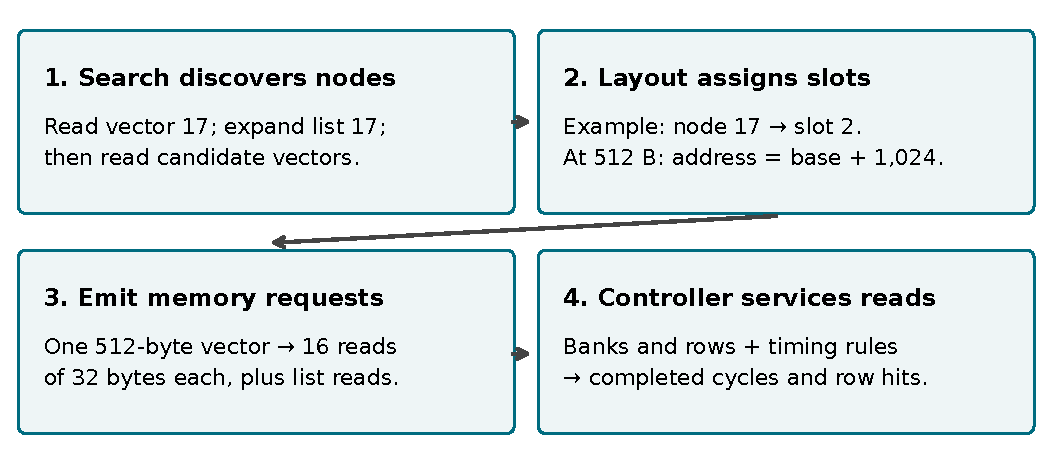
\includegraphics[width=\textwidth]{generated/study_pipeline.pdf}
\caption[The experiment pipeline]{From a graph search to a timing result. Node 17 and slot 2 are an illustrative example, not another measured experiment. Changing the layout changes the second stage while preserving the first.}\label{fig:pipeline}
\end{figure}

For example, suppose the logical search needs vectors 17 and 29 consecutively. One layout might place them in slots 2 and 3, and another in slots 2 and 4. At 512 bytes per vector and a 1-KiB aligned block, slots 2 and 3 share a block; slots 2 and 4 do not. Both searches still evaluate the same vectors and return the same answers. Their memory addresses differ, so the controller may require different commands or expose different bank overlap. This is the intervention the experiment isolates.

\begin{figure}[htbp]\centering
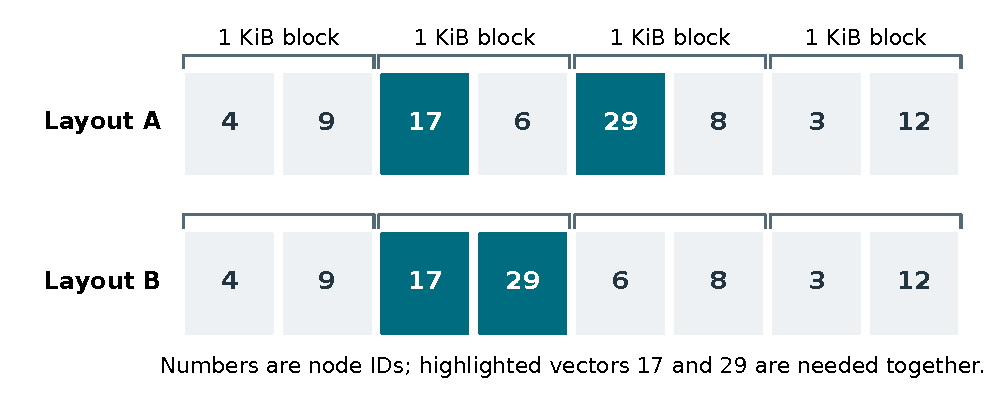
\includegraphics[width=\textwidth]{generated/layout_example.pdf}
\caption[Example of vector placement]{An illustrative excerpt of two vector layouts. Each vector occupies 512 bytes, so two fit in a 1-KiB block. Layout B puts the highlighted pair in one block while retaining every shown vector exactly once. That creates an opportunity for row reuse, but also concentrates the pair's requests in one bank.}\label{fig:layout-example}
\end{figure}

\section{Stock-search instrumentation}
The vendored search implementation contains observer calls immediately before vector distance reads and after determining an expanded list's length. Heap operations, candidate bounds, stopping conditions, and tie handling remain in stock search. The adapter snapshots adjacency for every graph level after construction and forwards observer records to a collector. The observer is cleared after successful and exceptional searches.

The maintained build disables optional CPU prefetching while retaining SIMD distance arithmetic and stock search decisions. Prefetches are speculative early memory requests, outside this demand-stream model. The remediation record documents the vendor safety issue that motivated disabling that implementation path.

Internal HNSW node numbers follow insertion order, while external corpus IDs must remain stable. The adapter translates internal IDs in observed accesses and adjacency lists back to corpus IDs. Tests check that translation against an independently built index after shuffled insertion. Thus changing construction does not silently change the meaning of identity placement or exact-neighbour IDs.

The adapter is single-threaded; the mutable observer is not a general concurrent-search interface. Tests compare results against a separately built stock index on continuous and tie-heavy inputs, with $\texttt{efSearch}=4$ and 64 and $k=10$. They also check entry-vector presence and list sizes. In every real evaluation query, instrumented and unobserved stock result lists must match exactly before the run continues.

Direct instrumentation is stronger than maintaining a second approximate implementation of the search algorithm, but still requires auditing the selected hooks. The instrumentation covers demand vector/list accesses. It does not turn hnswlib into a full CPU memory tracer.

\section{Address representation}
Let $b$ be the vector payload in bytes, $N$ the corpus size, and $B=32$ the native transaction size. Vectors occupy a dense separate array starting at $A_V=\mathtt{0x10000000}$:
\begin{equation}
 a_V(v)=A_V+\pi(v)b,\qquad A_V\leq a_V(v)<A_V+Nb.
\end{equation}
The adjacency region begins at the next transaction boundary after the vector end plus a 1-MiB separating gap. Every $(v,\ell)$ list receives its own aligned allocation in node/level order. Its payload is
\begin{equation}
 s_A(v,\ell)=4+4\,\deg(v,\ell),
\end{equation}
representing a four-byte header and four-byte neighbour IDs. The next list begins after rounding the current allocation end up to $B$. A 32-neighbour base list therefore occupies 132 payload bytes and reserves 160 bytes at 32-byte alignment. Distinct list allocations cannot overlap. The allocation is independent of vector layout for a given footprint.

For any payload beginning at $a$ with size $s$, the emitted transactions cover
\begin{equation}
 B\left\lfloor\frac{a}{B}\right\rfloor,\;B\left\lfloor\frac{a}{B}\right\rfloor+B,\ldots < a+s.
\end{equation}
This handles partial and unaligned payloads. It can read padding or the containing line of a neighbouring dense vector, but does not reuse a fetched line across logical records. There is no cache or duplicate-read coalescing. The two primary vector widths are multiples of 32, so their per-vector request count is layout-independent.

This separate-array representation is not hnswlib's native physical allocation. It isolates vector placement while holding adjacency placement fixed. An integrated reordered index would also need a mapping mechanism; mapping lookup traffic and storage overhead are outside the simulated stream. For non-identity layouts, the artifact stores both mapping directions as 64-bit entries, or $16N$ bytes, excluding container overhead. A deployed implementation could choose another representation, but cannot assume translation is free without justification.

\section{Verified HBM2 geometry}
\label{sec:geometry}
The simulator revision is \texttt{7bead6cb7c4b03e095c6d4769ae3181a8e0bf6da}. The primary preset is \texttt{HBM2\_8Gb} with \texttt{HBM2\_2000Mbps}. The actual hierarchy is one configured channel, two pseudochannels, two SIDs, four bank groups, four banks, 32,768 rows, and 128 column units. The preset exposes a 128-bit channel interface, but explicitly sets the data payload to 32 bytes for one pseudochannel. The mapper reduces the column count by the prefetch factor of four, giving 32 native transactions per bank-row address span.

The resulting contiguous same-bank, same-row span is $32\times32=1024$ bytes for the default mapper. Its bit decomposition is shown in Table~\ref{tab:bits}. Integration tests send sample addresses through the actual simulator and compare callback addresses with this decomposition, including a high address within the configured capacity. This avoids inferring geometry from a performance curve.

\begin{table}[htbp]\centering
\caption[Default address mapping]{Default \texttt{RoBaRaCoCh} mapping for one channel. Bit 0 is the least significant address bit.}\label{tab:bits}
\begin{tabular}{lrl}\toprule
Field & Address bits & Values\\\midrule
Byte within transaction & 0--4 & 32 bytes\\
Transaction column & 5--9 & 32 columns\\
Pseudochannel & 10 & 2\\
SID & 11 & 2\\
Bank group & 12--13 & 4\\
Bank & 14--15 & 4\\
Row & 16--30 & 32,768\\\bottomrule
\end{tabular}
\end{table}

The alternate \texttt{ChRaBaRoCo} mapper keeps column bits 5--9, places row in bits 10--24, then bank, bank group, SID, and pseudochannel in bits 25--30. It therefore presents very different bank parallelism for a small contiguous range despite retaining a 1-KiB row span. There is no interleaving across multiple configured channels in either experiment.

The preset's DRAM period is 1 ns at its stated 2,000-Mbps transfer rate. Several timing choices in upstream source are annotated as estimates. This work verifies trace interpretation, mapping, and accounting; it does not independently validate the preset against a physical HBM2 device.

\section{Frontend, concurrency, and completion}
\label{sec:frontend}
Each line has the form \texttt{LD address query kind}. The frontend accepts read-only, native-aligned addresses, requires monotonic query positions, and supports untagged microbenchmark lines as one query. It submits at most one transaction per configured issue interval and limits submitted-but-uncompleted requests. A rejected controller submission is retried without advancing the trace.

The controller implementation is \texttt{GenericDDR}, which selects at most one command per controller cycle. The HBM2 timing specification still constrains those commands, but this is not the specialised dual-command-issue HBM controller. This explicit choice limits claims about peak HBM utilisation.

The primary configuration permits 64 outstanding reads, a 32-entry read buffer, and one submission opportunity per memory cycle. These are separate constraints: active and pending controller state can make total in-flight traffic differ from the waiting read-buffer occupancy. The frontend uses completion callbacks to enforce the outstanding limit. The limit counts 32-byte transactions, not vectors: 64 transactions represent 2 KiB of payload, equivalent to four complete 512-byte vectors or sixteen 128-byte vectors before accounting for adjacency traffic. Changing footprint therefore changes both grouping capacity and how much logical vector work fits within this request bound.

At a query boundary, all earlier reads must complete before the next query can issue. Bank-row state remains warm, refresh continues during service, and there is no cache state to reset. The simulation starts with the default initial DRAM state. It terminates only when callbacks have arrived for every trace read. A watchdog rejects a nonterminating run.

The frontend's clock configuration is derived from the pinned simulation loop rather than assumed from parameter names. Its \texttt{clock\_ratio}=1 and the memory system's ratio equal to the issue interval produce one frontend opportunity every specified number of memory cycles. A four-cycle issue interval is tested as a sensitivity.

For each query, the frontend records the minimum accepted-request arrival and maximum read departure in controller cycles. Their difference is the query's stream service interval. Total controller cycles include the complete stream and refresh effects. Neither measure includes graph computations or the time to discover future addresses. An in-flight limit of one serialises memory requests but still does not add distance computation; it is a concurrency sensitivity, not a complete dependency-aware HNSW model.

\section{Page policy and scheduler settings}
The default policy is \texttt{Open}. Sensitivities use \texttt{ClosedCAP} with cap explicitly equal to one and four. A cap is the policy's column-access count within an activation; it is not a guarantee that every pending request is classified as a row miss. The controller can have multiple requests and commands in progress, and upstream row classification occurs when a request is first scheduled. All page-policy findings refer to these implementations.

The study also tests \texttt{FRFCFS-RowHit}, read-buffer capacity eight, outstanding limits one and 16, issue interval four, and the alternate mapper. Every setting first replays all five layouts at both footprints on the first held-out split. Three informative settings---one outstanding read, cap four, and the alternate mapper---are then repeated across all ten splits. The remaining settings retain their exploratory single-split status.

\chapter{Layouts, metrics, and correctness}
With the address representation fixed, the next choice is how to assign nodes to slots. The five layouts use progressively different information: corpus order, randomness, graph structure, and observed training searches. This chapter explains those choices and the measurements used to compare them.
\section{Baseline layouts}
\textbf{Identity} assigns slot $v$ to node $v$, preserving corpus order, including when graph insertion is shuffled. It is the practical reference for this separate-array representation, not a claim about the original allocator's addresses.

\textbf{Random} uses a seeded permutation of all nodes. It is a control for locality available from the other mappings, not an upper bound on irregularity. Its RNG varies with the evaluation split seed.

\textbf{BFS} (breadth-first search) visits a node's immediate neighbours before moving to the next graph frontier. It assigns slots in breadth-first order over the base graph, restarting from the lowest unplaced ID for disconnected regions. It may bring some graph neighbours close together, but cannot guarantee that all nodes expanded together share a row.

\textbf{Community} groups nodes by graph connectivity. Each node starts with a label; repeated updates favour labels common among its neighbours. This asynchronous label propagation runs for at most 20 iterations, then places communities contiguously. Community-size ties and within-community choices are deterministic under the configured seed. It is a lightweight structural heuristic rather than an exact graph-partitioning solver.

\section{Workload-trained greedy layout}
The \QA{} method asks which vectors tend to be read near one another during training searches. If nodes 17 and 29 often occur close together in those searches, it gives their pair a larger weight and tries to store them together. This can capture a relationship between two neighbours expanded from the same parent even when the two nodes do not have a direct graph edge. The held-out queries then test whether that training signal is useful beyond the searches used to build it.

Formally, the method learns a symmetric weighted co-visitation graph from training vector accesses. Within a query, each vector access contributes a weight increment with the different nodes in a bounded recent list. The default list capacity is 16 distinct nodes. A node already in that list contributes pairs but is not reinserted or refreshed in recency; the list is therefore a bounded distinct-history heuristic rather than a fixed number of access occurrences. Query boundaries reset the list.

After accumulation, each node's partners are sorted by descending weight, breaking ties by node ID. Seeds are sorted by total incident weight with the same deterministic ID tie-break. The layout places the first unplaced seed and then its heaviest unplaced partners that fit before the current physical block boundary. A short group may leave room for the next seed, but that next seed's partners may not spill into a subsequent block. Unplaced nodes are appended using BFS restarts.

The primary block size is the verified 1,024-byte contiguous row span. A footprint of 512 bytes gives capacity for two complete vectors in an aligned block; 128 bytes gives eight. For example, if a 512-byte block group starts at slot 2, only one partner fits beside the seed before slot 4 begins the next block. At 128 bytes, a fresh aligned block can hold the seed and seven partners. The mapping is rebuilt separately for each footprint. A 2,048-byte grouping is tested as a heuristic sensitivity, without calling it the physical HBM2 row span.

The method optimises a proxy: temporal co-visitation in a finite training sample. It does not know controller command timing or adjacency interference, and does not minimise simulated cycles directly. Low coverage, the weighting rule, greedy ordering, and the grouping objective can each limit its performance. A loss by this method would not prove that the workload has no useful placement information.

\section{Metrics and their meanings}
\subsection{Search accuracy and traffic}
For each test query, exact squared distances are evaluated over exactly the indexed base subset, using double accumulation and distance/ID sorting. Recall is computed against those IDs. Full-million-vector ground truth is not used for the 100k index. The SIFT components have integral values in the mirrored float representation, which also makes the recorded tie convention interpretable.

Vector and adjacency logical records, their graph levels, emitted read count, allocated address bounds, construction times, split membership, returned IDs, and truth IDs are retained. Upper-layer records constitute \UpperFraction\% of logical evaluation records on average. They are included in timing rather than discarded on the assumption that they are negligible.

\subsection{Address-colocation diagnostics}
Let $v_1,\ldots,v_m$ denote one query's vector records in order, after skipping consecutive repeated node IDs for the transition count. For block size $R$, define
\begin{equation}
 g(v)=\left\lfloor\frac{\pi(v)b}{R}\right\rfloor.
\end{equation}
The \emph{consecutive-vector same-block fraction} counts transitions for which $g(v_i)=g(v_{i+1})$, divided by all eligible within-query transitions, then aggregates counts across queries. It compares vector starts, not all bytes of a potentially crossing vector. It resets between queries and ignores adjacency records by definition.

A second diagnostic takes each query's unique visited-node set and counts pairs sharing a start-address block. This co-visit same-block fraction is computed using per-block counts, avoiding explicit quadratic enumeration. Both diagnostics are address statistics. They do not include bank state, intervening adjacency requests, controller reordering, or command timing. They must not be labelled measured DRAM row-hit rates.

\subsection{Simulator outputs}
The primary performance quantity is completed-stream controller cycles. The simulator's read row-hit fraction is
\begin{equation}
 H=\frac{n_{\mathrm{hit}}}{n_{\mathrm{hit}}+n_{\mathrm{miss}}+n_{\mathrm{conflict}}}.
\end{equation}
The three counters classify requests in the pinned controller. They are not an application speedup and need not track cycles monotonically. Raw controller statistics include latency and throughput values, but the thesis's headline comparison uses cycles and conserved traffic, avoiding an inference from a more visually separated proxy.

\section{Maintained checks}
Table~\ref{tab:checks} describes invariants checked by the artifact. Tests target failure modes that can change the scientific comparison; the numerical direction of a layout result is not made a test requirement.
\begin{table}[htbp]\centering\small
\caption[Correctness checks]{Correctness checks required before analysing results.}\label{tab:checks}
\begin{tabular}{p{0.29\textwidth}p{0.62\textwidth}}\toprule
Area & Check\\\midrule
Search & 800 independent-index result comparisons across corpus/shuffled insertion, including ties and $\mathrm{ef}<k$; per-query instrumented/unobserved equality in every real run.\\
Address space & All adjacency levels have separate aligned ranges; known 132-byte lists cannot alias; partial payloads emit every touched transaction.\\
Placement & Every mapping is a bijection with a valid inverse; footprint-specific constructions and partial-group boundaries have regression cases.\\
Metrics & A vector in each of two separate queries cannot create a within-query transition; known same-block examples produce the expected count.\\
Input & Empty, short, ragged, nonfinite and truncated records fail; numeric overflow and negative parameters fail in maintained trace tools.\\
Frontend & Native transaction size and mapper samples match the actual configuration; outstanding limits and query drain are checked; a one-read trace completes.\\
Accounting & Trace lines, submitted reads, completed callbacks, served reads, and classified reads must agree for every analysed run.\\
Quality sweep & Slots remain unique and the address multiset is identical at every quality setting; observed fixed slots match the requested integer count.\\\bottomrule
\end{tabular}
\end{table}

\chapter{Experimental protocol}
A fair comparison needs more than several layout implementations. It needs the same search work, a clear accuracy check, disjoint training and evaluation, and repetitions that vary the intended source of uncertainty. The protocol first tests controlled streams, then actual HNSW demands, and finally the assumptions on which the comparison depends.
\section{Data, construction, and held-out queries}
The SIFT source is the ANN-Benchmarks HDF5 mirror \cite{annbench,pq}. The artifact records its SHA-256 digest, converts the first 100,000 training vectors to fvecs, and converts all 10,000 query vectors. Corpus IDs are the zero-based prefix positions. The mirror calls corpus data ``train and query data ``test; those names are separate from this thesis's training/test partition of the query pool. Query IDs are retained after shuffling; vector dimensions and finite components are checked.

For each of ten split seeds, a permutation of the fixed 10,000-query pool determines the split. The first 500 queries train the co-visitation model; the last 200 evaluate every layout. This convention keeps the same test queries when training size changes and leaves training and testing disjoint. Repetitions hold the corpus, insertion order, HNSW parameters, and index seed 100 fixed. They vary training/test selection and the random/community layout seeds. They do not quantify index-construction variation or alternative corpus subsets.

Index reconstruction uses the same deterministic insertion protocol in each process. Corpus and trace hashes, parameters, query IDs, and mappings identify the experiment. Results describe this fixed graph and query pool. New datasets or index seeds would be required for broader ANN conclusions.

\section{Two different kinds of repetition}
A random seed makes a pseudo-random procedure reproducible. It does not specify what source of variation is being tested. The primary ten seeds change which queries train and evaluate a layout, while keeping the graph fixed. The added construction study changes graph seeds to 101 and 102 while retaining corpus order, and separately uses graph seed 100 with shuffled insertion order seeded by 17. Each of these three additional graphs uses query splits one through three. The original graph on those same three splits supplies the reference.

Corpus IDs and the exact-neighbour search universe remain fixed. Layouts are compared within a graph and split; raw times across different graphs also reflect different search work. Graph and insertion-order hashes verify that the intended graph is reused across its splits and that the selected constructions differ. With only three deliberately selected alternatives, their results are reported as observed means and ranges, not as a confidence interval over all possible graphs.

\section{Paired uncertainty}
For split $s$ and layout $L$, let $T_{s,L}$ be completed-stream cycles at one fixed footprint. The paired relative difference against BFS is
\begin{equation}
 d_{s,L}=100\left(\frac{T_{s,L}}{T_{s,\mathrm{BFS}}}-1\right).
\end{equation}
For example, 99,700 cycles against a 100,000-cycle BFS run gives $d=-0.3\%$: fewer cycles is a negative difference. Each comparison uses the same queries and graph, so a difficult query set cannot make one layout look worse simply because it was tested on more work. The estimate is the mean of these ten differences. The reported interval is
\begin{equation}
 \bar d_L\;\pm\;t_{0.975,9}\frac{s_d}{\sqrt{10}},\qquad t_{0.975,9}\approx2.262,
\end{equation}
using the conventional Student interval \cite{student}. The sampling unit is an independently selected split/layout RNG condition within the fixed pool. The interval expresses uncertainty in the mean effect under this protocol; it is not a range that should contain 95\% of individual query latencies. Query sets may overlap between repetitions; there is no leakage between training and testing within one split. The interval describes variability induced by that random protocol, conditional on the corpus, graph and simulator.

The simulator is deterministic for a fixed trace and configuration; rerunning identical inputs would not measure workload uncertainty. Individual queries are not treated as independent hardware replications, and overlap of marginal layout intervals is not used as a test of a paired difference. These are exploratory 95\% intervals for individual comparisons, without a family-wise multiplicity correction. An interval containing zero is inconclusive about the sign at this precision; it is not evidence of equivalence. No equivalence margin is specified, and the study makes no statistical-equivalence claim.

\section{Controlled microbenchmarks}
The ordering experiment reads 4,096 vectors with 128-byte payloads, producing 16,384 native transactions. Sequential and permuted variants have identical address multisets. Request presorting stably sorts disjoint batches of 1, 16, 64, 256, 1,024, 4,096, or 16,384 \emph{transaction records}. These are not sliding windows or numbers of vectors. The full-size sort is checked to reproduce the sequential trace byte for byte.

The run-length generator visits contiguous groups in shuffled group order. Run lengths are 1, 2, 4, 8, 16, 32, and 64 vectors. Payload widths are 96, 128, 192, 256, 384, and 512 bytes; base offsets relative to the aligned base are 0, 32, and 480 bytes. A smaller run/mapping matrix also tests the alternate mapper. The generator evaluates available locality, not attainable HNSW placement.

The placement-quality intervention holds the logical contiguous-group visits fixed at 16 vectors per group. For requested quality $q$, exactly $N-\lfloor Nq/100\rfloor$ IDs are selected and their slots cyclically permuted. All other IDs keep their original slot. The special impossible case of exactly one displaced slot is rejected. Thus ``quality'' means fixed \emph{slot} fraction, not fixed row or cluster fraction. The tested percentages are 0, 25, 50, 75, 90, and 100.

\section{Sensitivity and preprocessing cost}
The real-data sensitivity matrix changes one controller setting at a time on split one. Training-size ablations use 100 and 1,000 queries; window ablations use four and 64 distinct-history entries; block-size sensitivity uses 2 KiB. Their test IDs remain the same, and BFS and \QA{} are both replayed at both footprints.

The driver times index construction, training-query collection, co-visitation construction, and each layout build using a steady clock. These are wall-clock observations on a shared execution environment, with other experiment processes potentially active. They establish that preprocessing is nonzero and expose order-of-magnitude costs. They are not controlled hardware throughput benchmarks or a measured amortisation break-even point.

\chapter{Results}
\label{ch:results}
The results follow the argument from a simple case to a realistic access pattern. Controlled streams first reveal why locality and timing can disagree. The SIFT experiment then measures how much the tested layouts change service at fixed search work. Repeated controller settings, graph variations and command diagnostics examine how stable those differences are and why they arise.
\section{Ordering: row hits and cycles can disagree}
Figure~\ref{fig:order} begins with the simplest controlled comparison: two orders of the same reads. Sequential service takes \SequentialCycles{} cycles at \SequentialHit\% classified row hits. The permuted stream takes \RandomCycles{} cycles at \RandomHit\% hits. Every stream read completes and is represented in the classification counters.

The sequential sequence has a higher hit fraction but takes more cycles at the default concurrency. This result is compatible with the different banks exposed by the request order: with the default mapping, 32 adjacent transactions fill one row span, so a 64-request contiguous prefix exposes only two bank instances, whereas scattered vectors can expose more. The exact performance follows from scheduling, buffers, and timing together. Row-hit fraction alone does not isolate the cause or establish a necessary condition for good service.

At outstanding limit one, full sorting changes the permuted stream's 398,592 cycles to 325,786 cycles. This comparison is retained in the raw sensitivity results and demonstrates that available concurrency materially changes the ordering result. It does not add HNSW's compute dependencies.

\begin{figure}[htbp]\centering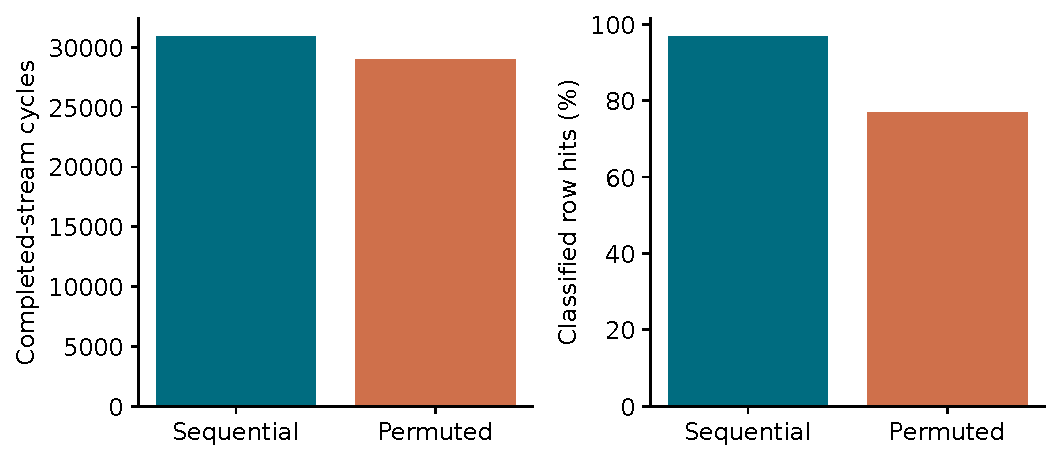
\includegraphics[width=\textwidth]{generated/micro_order.pdf}
\caption[Row hits and service cycles]{Default native-transaction microbenchmark. Higher row-hit fraction does not imply fewer completed-stream cycles.}\label{fig:order}\end{figure}

\subsection{Following the commands rather than the proxy}
The next step is to ask what the controller actually does. The pinned simulator provides observers that count each issued command and, for the microbenchmark, record its cycle and decoded address. Replaying with these observers gives exactly the same cycles and row-hit counts as the original runs. The observers add evidence without changing the simulated schedule.

Table~\ref{tab:microcommands} gives an exact accounting for this controller. Because it selects at most one command per cycle,
\begin{equation}
 T = N_{\text{command cycles}} + N_{\text{no-command cycles}}.
\end{equation}
A command cycle may open or close a row, issue a read, or perform refresh. A no-command cycle can arise from timing restrictions, a lack of eligible work, or draining the last reads. It is deliberately not labelled as a particular stall cause.

\begin{table}[htbp]\centering\small
\caption[Command accounting for request order]{Controlled ordering experiment with command observers. ACT opens a row; PRE combines per-bank and all-bank precharge commands. The read count is 16,384 in every row. ``Limit'' is the maximum number of outstanding reads.}\label{tab:microcommands}
\begin{tabular}{rlrrrr}
\toprule
Limit & Order & Cycles & ACT & PRE & No command \\
\midrule
64 & Sequential & 30894 & 528 & 38 & 13930 \\
64 & Permuted & 28968 & 3793 & 3319 & 5458 \\
1 & Sequential & 325786 & 588 & 166 & 308482 \\
1 & Permuted & 398592 & 4044 & 1135 & 376825 \\
\bottomrule
\end{tabular}

\end{table}

At limit 64, the permutation opens and closes more rows, yet has fewer no-command cycles. The reduction in those cycles exceeds the cost of the extra command-issue cycles. At limit one, no other read can hide the waiting for the current read, and the additional row changes make permutation slower. The two interventions expose the trade-off: reducing commands and overlapping service are different ways to reduce time.

The offered sequential stream spans an average of \SequentialBanks{} different bank instances per sliding window of 64 requests, compared with \RandomBanks{} for the permutation. Each statistic counts complete windows within queries under the verified default mapper. This measures diversity in the input stream; it is not a measurement of how many banks are ready simultaneously, or how many requests occupy the controller queue.

\begin{figure}[htbp]\centering
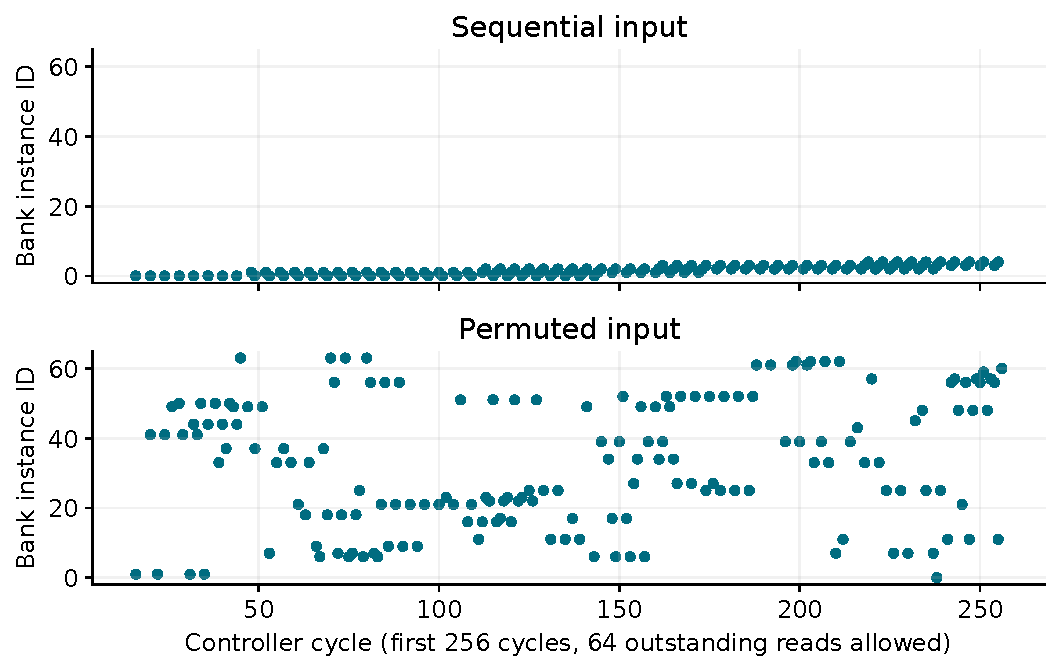
\includegraphics[width=\textwidth]{generated/command_timeline.pdf}
\caption[Read-command timing and bank exposure]{Actual read-command issues in the first 256 controller cycles, with limit 64. Each dot is one RD command; the vertical position identifies its bank instance. Sequential requests concentrate early service in a few banks, while the permutation exposes a wider set. The full-run counts, rather than this short initial interval alone, support the timing comparison.}\label{fig:commands}
\end{figure}

This evidence supports a locality--parallelism explanation for the controlled reversal. It does not assign every saved cycle to an individual timing rule: refresh, buffering and scheduling interact. The important result is that an observed reduction in row operations can be outweighed by the service opportunities lost elsewhere in the schedule.


\section{Finite request presorting}
\begin{table}[htbp]\centering\caption[Request-presorting windows]{Disjoint presorting windows on the permuted 16,384-request trace. The full window exactly reproduces the sequential trace.}\label{tab:reorder}
\begin{tabular}{lrr}
\toprule
Window (requests) & Cycles & Hit (\%) \\
\midrule
1 & 28968 & 76.85 \\
16 & 28950 & 76.92 \\
64 & 28961 & 76.90 \\
256 & 28912 & 77.15 \\
1024 & 28728 & 79.80 \\
4096 & 27001 & 88.70 \\
16384 & 30894 & 96.78 \\
\bottomrule
\end{tabular}
\end{table}
Table~\ref{tab:reorder} reports the tested windows. Sorting can expose a different issue order than the original permutation, and can also reduce bank diversity. Sorting the whole known stream places its addresses in exactly the sequential order; the byte-for-byte trace check verifies this endpoint. Its feasibility during an actual dependent graph search is a separate question: the required future addresses may not yet be known.

The artifact also repeats selected windows with explicit row-hit-prioritising scheduling and with one outstanding request. Those experiments test the controller explanation rather than presuming that all software sorting duplicates FRFCFS. They do not justify a general claim that software reordering is useless or that the largest sorting window is useful in a deployed ANN implementation.

\section{Contiguous runs, alignment, and placement quality}
Figure~\ref{fig:runs} separates hit-fraction behaviour from cycle behaviour. To summarise hit saturation on the finite grid, the threshold is the smallest tested run length for which that point and every larger tested point are within one percentage point of the best hit fraction in the same width/offset sweep. Table~\ref{tab:threshold} reports the resulting run \emph{bytes}. This is an empirical finite-grid summary, not a physical-law fit or a guarantee about untested run lengths.

\begin{figure}[htbp]\centering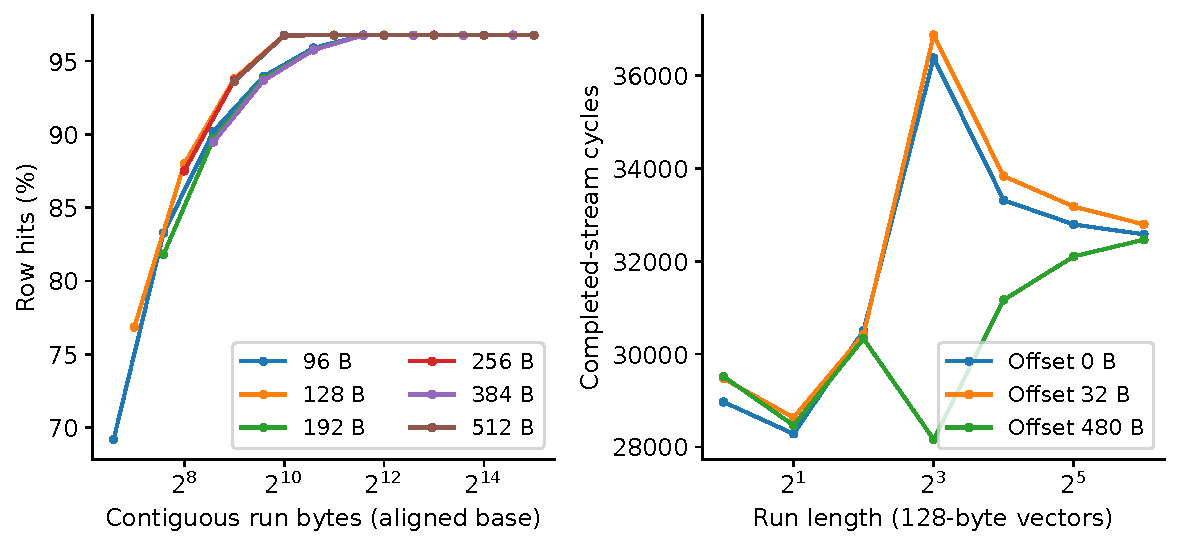
\includegraphics[width=\textwidth]{generated/run_sensitivity.pdf}
\caption[Contiguous runs and alignment]{Contiguous-run sensitivity to payload width and alignment. The left panel measures classified hits; the right panel shows that cycle behaviour requires separate examination.}\label{fig:runs}\end{figure}
\begin{table}[htbp]\centering\caption[Empirical run-byte thresholds]{Run-byte threshold for sustained hit fraction within one percentage point of the best tested point, by base offset. The threshold is conditional on this grid and configuration.}\label{tab:threshold}
\begin{tabular}{lrrr}
\toprule
Vector bytes & Offset 0 & Offset 32 & Offset 480 \\
\midrule
96 & 1536 & 3072 & 3072 \\
128 & 1024 & 4096 & 4096 \\
192 & 1536 & 3072 & 3072 \\
256 & 1024 & 4096 & 4096 \\
384 & 3072 & 3072 & 3072 \\
512 & 1024 & 4096 & 4096 \\
\bottomrule
\end{tabular}
\end{table}

The 1-KiB contiguous row span is independently established by address decoding. A saturation threshold can be larger, smaller in a particular grid, or affected by alignment and the controller's request mix. It should not be used to infer the row size after the fact. The alternate mapping experiments additionally change the bank opportunities associated with a contiguous address range. A predictive universal byte-budget rule is not established.

Figure~\ref{fig:quality} and Table~\ref{tab:quality} use only bijective layouts with identical address multisets. Reducing the fixed-slot fraction can move a vector within or across its original bank-row group, so the percentage is not a direct measurement of retained row locality. The curve describes this chosen corruption process. The experiment measures robustness to this specific perturbation. Translating a fixed-slot percentage into an acceptable engineering threshold would require a target cycle benefit and a preprocessing-cost model.
\begin{figure}[htbp]\centering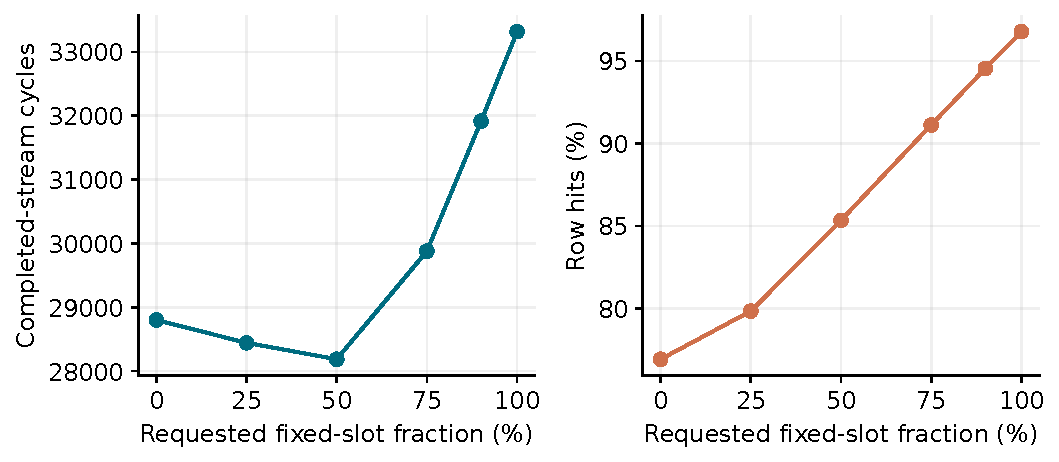
\includegraphics[width=\textwidth]{generated/quality.pdf}
\caption[Placement perturbation]{Valid fixed-slot-quality experiment. Each condition retains all 4,096 storage slots exactly once.}\label{fig:quality}\end{figure}
\begin{table}[htbp]\centering\caption[Placement-quality measurements]{Placement-quality results under the specified cyclic displacement process.}\label{tab:quality}
\begin{tabular}{lrr}
\toprule
Fixed slots (\%) & Cycles & Hit (\%) \\
\midrule
0 & 28801 & 76.92 \\
25 & 28443 & 79.84 \\
50 & 28186 & 85.34 \\
75 & 29880 & 91.11 \\
90 & 31915 & 94.54 \\
100 & 33316 & 96.77 \\
\bottomrule
\end{tabular}
\end{table}

\section{Held-out SIFT comparison}
Table~\ref{tab:real} contains the real timing comparison and both locality measures. Mean Recall@10 is \SiftRecall\%, with the split-level interval [\SiftRecallLow, \SiftRecallHigh]\%. Within a split all five layouts have exactly the same logical query result and the same emitted read count at a given footprint. The table's differences therefore reflect the modelled placement and controller interactions rather than a changed number of HNSW distance evaluations.

\begin{table}[htbp]\centering\small
\caption[Paired SIFT layout comparison]{Ten paired SIFT100k splits. Cycles are mean totals for 200 held-out queries. Hit is the simulator classification fraction; block is the consecutive-vector same-block diagnostic. The final column is mean relative cycle difference and its paired 95\% interval; negative is faster than BFS.}\label{tab:real}
\resizebox{\textwidth}{!}{\begin{tabular}{lrrrrr}
\toprule
Bytes & Layout & Cycles ($10^6$) & Hit (\%) & Block (\%) & $\Delta$ vs. BFS (\%) \\
\midrule
512 & Identity & 6.2322 & 93.24 & 0.02 & +0.30 [+0.24, +0.36] \\
512 & Random & 6.2327 & 93.24 & 0.00 & +0.31 [+0.12, +0.49] \\
512 & BFS & 6.2138 & 93.40 & 0.77 & +0.00 [+0.00, +0.00] \\
512 & Community & 6.2233 & 93.26 & 0.03 & +0.15 [+0.01, +0.29] \\
512 & Query-aware & 6.1943 & 93.62 & 1.02 & -0.31 [-0.37, -0.26] \\
128 & Identity & 1.6051 & 74.69 & 0.10 & +2.68 [+2.60, +2.76] \\
128 & Random & 1.6089 & 74.54 & 0.01 & +2.92 [+2.80, +3.04] \\
128 & BFS & 1.5632 & 76.47 & 1.68 & +0.00 [+0.00, +0.00] \\
128 & Community & 1.6000 & 74.83 & 0.21 & +2.35 [+2.17, +2.53] \\
128 & Query-aware & 1.5659 & 77.85 & 4.12 & +0.17 [+0.11, +0.24] \\
\bottomrule
\end{tabular}
}
\end{table}
\begin{figure}[htbp]\centering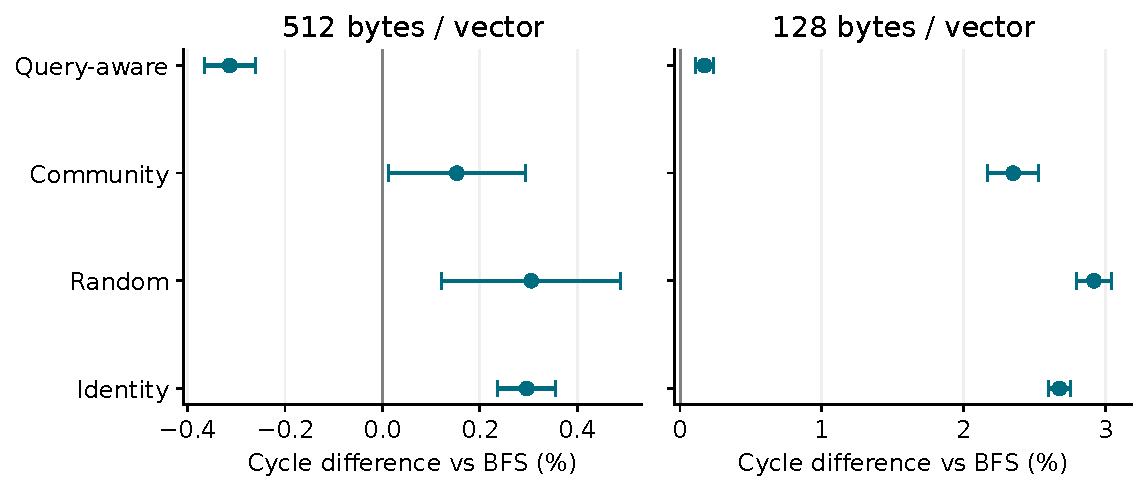
\includegraphics[width=\textwidth]{generated/real_paired.pdf}
\caption[Paired layout differences and uncertainty]{Paired cycle differences relative to BFS. Intervals describe query-split and random-layout variability on a fixed corpus/index/model.}\label{fig:paired}\end{figure}

For 512-byte vectors the \QA{} difference is \QADeltaFloat\% [\QALowFloat, \QAHighFloat]; for the hypothetical 128-byte footprint it is \QADeltaCompact\% [\QALowCompact, \QAHighCompact]. The footprint-specific mapping is rebuilt to match the number of vectors that fit in each grouping block. However, the 128-byte case still retains float32 traversal and recall. Its result cannot be promoted to evidence about PQ accuracy, quantised traversal, or distance-kernel speed.

The pairing matters because query difficulty changes the total traffic and cycles across splits. Comparing layout totals from unrelated query sets would confound the intervention. The original layout is included because a gain over a random permutation alone does not establish a benefit relative to the storage order available to a user.

\section{Controller and heuristic sensitivity}
Figure~\ref{fig:sensitivity} compares layouts under the one-setting-at-a-time controller matrix. Each cell is a relative cycle difference against BFS in the \emph{same} condition and split. The heat map should not be read as independent evidence from ten repetitions for each cell. It shows how a finding can change when the issue model or bank mapping changes.

\begin{figure}[p]\centering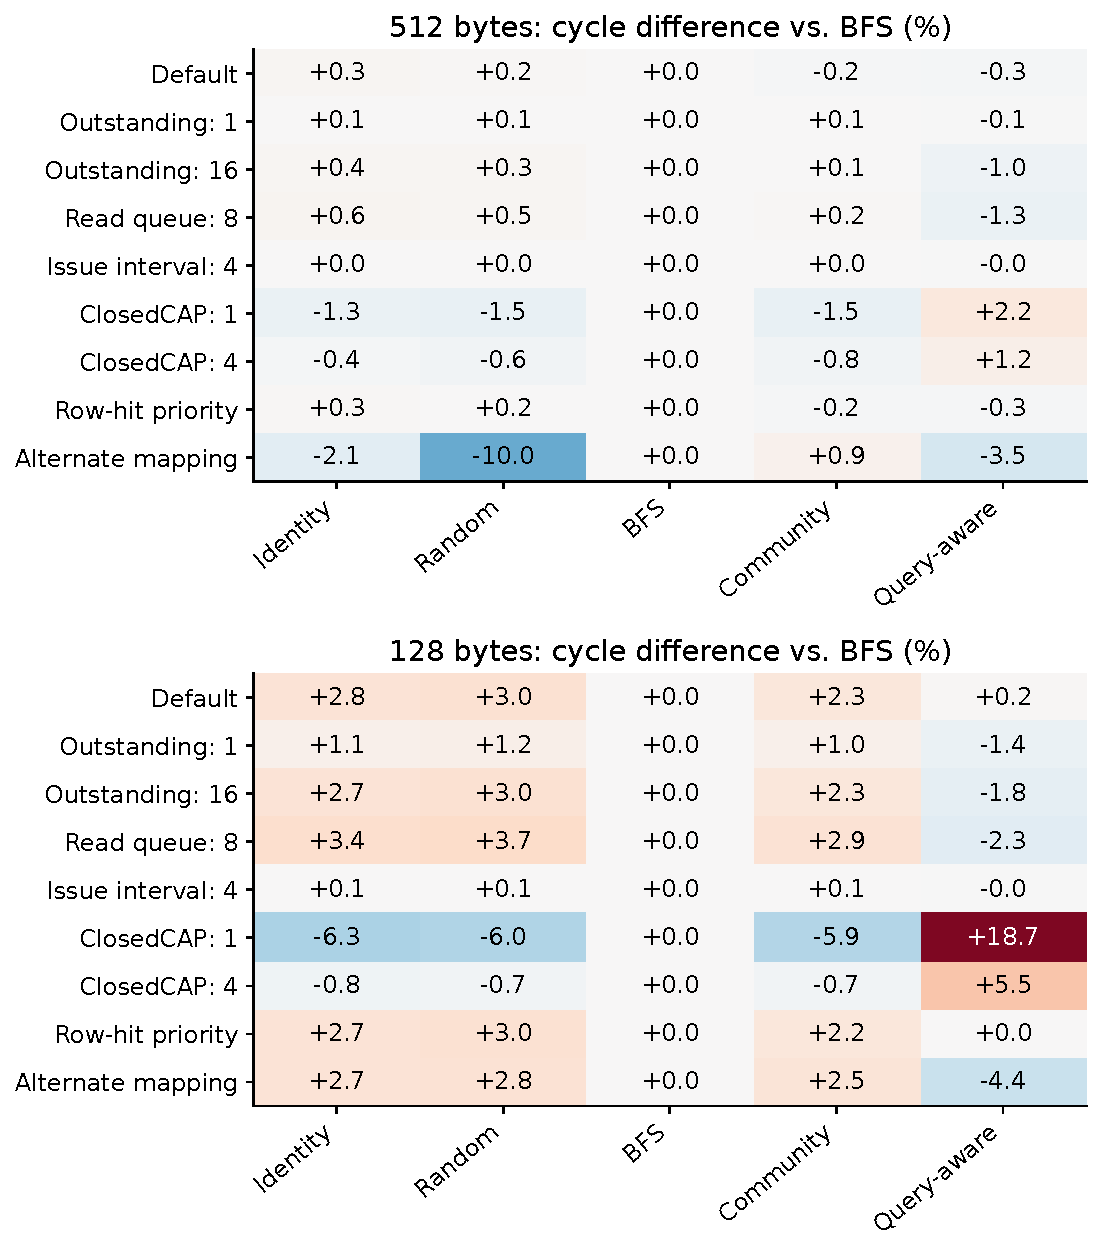
\includegraphics[width=\textwidth]{generated/sensitivity.pdf}
\caption[Exploratory controller sensitivity]{Split-one controller sensitivity. Values are cycle differences in percent against BFS; negative is fewer cycles. The two footprints use separately rebuilt layouts.}\label{fig:sensitivity}\end{figure}

The sensitivity matrix reverses some layout comparisons. For example, the workload-trained layout is faster than BFS with one outstanding request at both footprints, but slower under both capped policies. The alternate mapper favours it relative to BFS at both footprints in this split, although random placement is faster still for 512-byte vectors. These observations show dependence on the memory model; they are not additional ten-split estimates.

The cap-one policy and cap-four policy are explicitly different. In the controlled ordering traces, cap one gives sequential 146,441 cycles and random 33,798 cycles, while their classified hit fractions remain close to 50\%; cap four gives 63,333 and 29,708 cycles. These counters follow the simulator's scheduling-time classification and must not be interpreted as a guarantee that cap one produces zero classified hits. The much larger cycle separation demonstrates why a page-policy label or hit fraction is insufficient to predict service. The real-layout matrix supplies the relevant direct comparison; no claim that all placement benefit requires an open-page controller follows from the synthetic pair alone.

The ablations also change the sign of the comparison: the four-entry history loses to BFS at both widths, while 1,000 training queries give the workload-trained layout fewer cycles at both widths in this split. More training is not uniformly better for every footprint. These tests support examining the heuristic's objective and capacity rather than attributing all performance to static graph locality.

Table~\ref{tab:ablations} changes the heuristic's training and grouping parameters while retaining the test queries. Mean test vector-access coverage by the default training set is \MeanCoverage\%. Coverage here counts accesses whose node appeared in training, not the fraction of all corpus nodes or the fraction of learned edges shared with the graph. The ablations can reveal a limitation of this heuristic, but do not establish why every possible workload-trained placement would succeed or fail.

\begin{table}[htbp]\centering\small\caption[Training and grouping ablations]{Split-one heuristic ablations. Coverage is the fraction of test vector accesses to a node seen in training; model time excludes search collection and layout construction.}\label{tab:ablations}
\begin{tabular}{lrrrr}
\toprule
Condition & Bytes & $\Delta$ QA/BFS (\%) & Coverage (\%) & Model (s) \\
\midrule
train100 & 512 & -0.53 & 71.2 & 1.737 \\
train100 & 128 & +0.76 & 71.2 & 1.737 \\
train1000 & 512 & -0.26 & 99.7 & 24.494 \\
train1000 & 128 & -0.11 & 99.7 & 24.494 \\
window4 & 512 & +0.57 & 97.6 & 2.565 \\
window4 & 128 & +0.93 & 97.6 & 2.565 \\
window64 & 512 & -0.39 & 97.6 & 48.466 \\
window64 & 128 & +0.25 & 97.6 & 48.466 \\
block2048 & 512 & +0.24 & 97.6 & 11.249 \\
block2048 & 128 & +0.49 & 97.6 & 11.249 \\
\bottomrule
\end{tabular}
\end{table}

\section{Repeating the controller comparisons}
The exploratory matrix identifies informative changes, but a single split cannot show their variability across query samples. We therefore repeat three settings on all ten primary splits: one outstanding read, ClosedCAP cap four, and the alternate address mapper. These change the opportunity for overlap, row lifetime and address-to-bank placement respectively. Each setting replays all five layouts at both footprints, for 300 additional runs.

\begin{table}[htbp]\centering\small
\caption[Repeated controller comparisons]{Query-aware cycle difference against BFS under three repeated controller settings. Each estimate uses ten matched splits with the same graph. Negative means fewer cycles.}\label{tab:repeated}
\begin{tabular}{lrrr}
\toprule
Setting & Bytes & $\Delta$ QA/BFS (\%) & 95\% interval \\
\midrule
Outstanding: 1 & 512 & -0.13 & [-0.14, -0.13] \\
Outstanding: 1 & 128 & -1.26 & [-1.30, -1.21] \\
ClosedCAP, cap 4 & 512 & +0.89 & [+0.79, +0.99] \\
ClosedCAP, cap 4 & 128 & +5.27 & [+5.15, +5.39] \\
Alternate mapper & 512 & -4.02 & [-4.28, -3.75] \\
Alternate mapper & 128 & -4.12 & [-4.26, -3.99] \\
\bottomrule
\end{tabular}

\end{table}
\begin{figure}[htbp]\centering
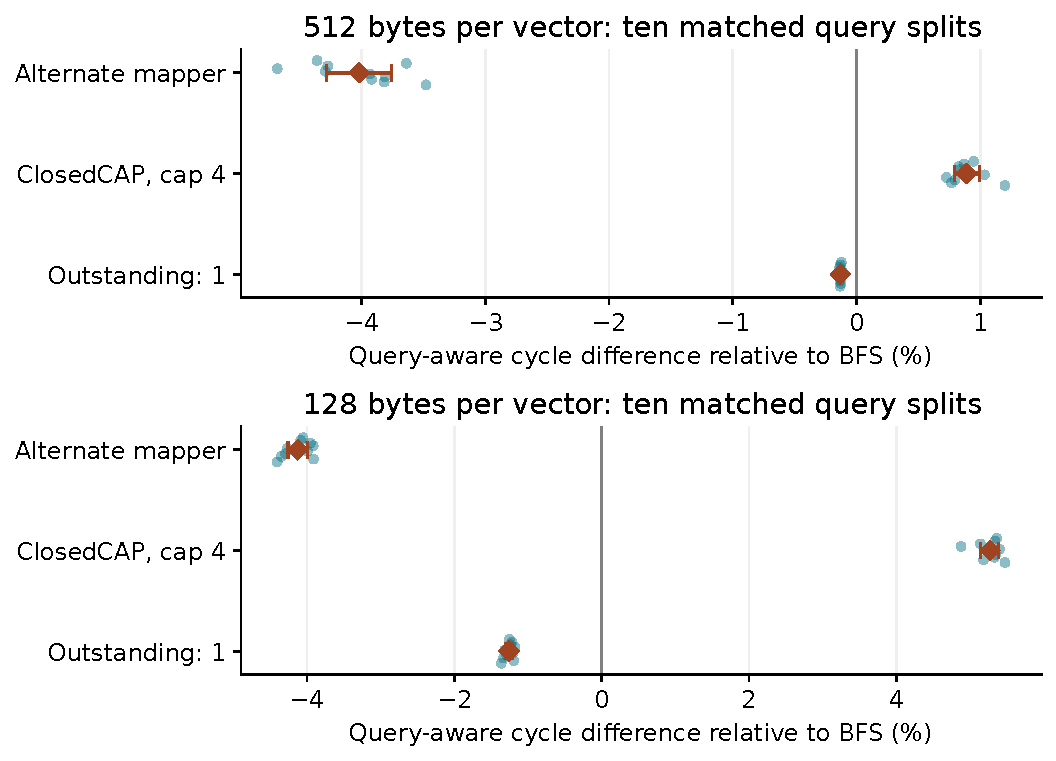
\includegraphics[width=\textwidth]{generated/robust_controllers.pdf}
\caption[Individual effects and paired intervals]{Individual split effects (small teal points) and mean with paired 95\% interval (orange diamond and bar). Showing the observations alongside the intervals makes their consistency and dispersion visible.}\label{fig:repeated}
\end{figure}

The query-aware/BFS sign is consistent across all ten splits in each repeated setting: query-aware is faster at both widths with one outstanding read and with the alternate mapper, and slower at both widths under cap four. The size of the effect also changes substantially, as Table~\ref{tab:repeated} shows. Under the alternate mapper, random placement is faster still than query-aware at 512 bytes in every split. A gain relative to BFS therefore does not identify the best layout among all controls.

The other controller settings and all training ablations retain their single-split interpretation. The repeated settings were chosen after inspecting the exploratory matrix; their ten splits include that original first split. This is a targeted robustness extension, not an independent confirmatory experiment. It strengthens the comparison under those specific interventions without sampling an architectural population.

\section{Changing the graph while preserving corpus IDs}
The previous repetitions share one constructed graph. The next experiment keeps the same 100,000 vectors but changes the structure used to search them. Graph seeds 101 and 102 vary HNSW's random construction with corpus insertion order fixed. A third alternative keeps graph seed 100 and shuffles insertion with seed 17. Each alternative uses query splits one through three and all five layouts at both footprints, adding 90 replays.

\begin{table}[htbp]\centering\small
\caption[Graph-construction robustness]{Query-aware/BFS cycle differences for four constructions on the same three query splits. The mean and minimum/maximum describe these observations; the range is not a confidence interval over possible graphs.}\label{tab:graphrobust}
\begin{tabular}{lrrr}
\toprule
Graph construction & Bytes & Mean $\Delta$ (\%) & Observed range (\%) \\
\midrule
Seed 100, corpus order & 512 & -0.341 & [-0.357, -0.331] \\
Seed 100, corpus order & 128 & +0.119 & [+0.034, +0.186] \\
Seed 101, corpus order & 512 & -0.247 & [-0.386, -0.062] \\
Seed 101, corpus order & 128 & -0.191 & [-0.267, -0.081] \\
Seed 102, corpus order & 512 & -0.268 & [-0.330, -0.212] \\
Seed 102, corpus order & 128 & -0.705 & [-0.798, -0.627] \\
Seed 100, shuffled order & 512 & -0.320 & [-0.499, -0.161] \\
Seed 100, shuffled order & 128 & +0.040 & [-0.057, +0.203] \\
\bottomrule
\end{tabular}

\end{table}

At 512 bytes, query-aware placement uses fewer cycles than BFS in every tested construction/split pair. At 128 bytes, the ranking changes: the reference graph's three-split mean is \GraphRefCompact\%, while seeds 101 and 102 give \GraphOneCompact\% and \GraphTwoCompact\%. Shuffled insertion has mean \GraphShuffleCompact\% and individual splits on both sides of zero. Thus the original 128-byte loss is not a stable property of the footprint alone. Query-split precision on one graph did not establish robustness to constructing another graph.

The reference row uses only those same three splits, making it comparable with the alternatives. Graph hashes confirm four distinct topologies, and repeated builds of each construction agree. Corpus IDs remain stable: changing insertion order does not redefine which vector a logical ID names, which vectors count as exact neighbours, or what identity placement means.

Recall across these graph/split conditions ranges from \GraphRecallMin\% to \GraphRecallMax\%. A changed graph can change the number of candidate evaluations and therefore total traffic. For this reason, Table~\ref{tab:graphrobust} compares layouts within each graph and split. Directly comparing absolute cycles from two different graphs would combine search-work and placement effects. These selected constructions expand the evidence beyond one topology, while leaving corpus and dataset generalisation open.

\section{Explaining the 128-byte layout reversal}
The main SIFT table contains a smaller version of the controlled paradox: query-aware placement gives more row hits than BFS at 128 bytes, yet slightly more cycles. To inspect that result, the command observers replay split one for both layouts with outstanding limits one and 64. Each case is run with the original mixed trace, vector requests only, and adjacency requests only. Query boundaries are preserved. Removing a request type is a diagnostic intervention, not an alternative complete HNSW execution.

\begin{table}[htbp]\centering\small
\caption[Command accounting for the layout reversal]{Query-aware minus BFS for the 128-byte diagnostic streams on split one. Negative counts mean fewer cycles or commands. The last two columns sum exactly to the cycle difference. Limit is the outstanding-read bound.}\label{tab:realcommands}
\begin{tabular}{rlrrrr}
\toprule
Limit & Stream & $\Delta$ cycles & $\Delta$ ACT & $\Delta$ commands & $\Delta$ no cmd. \\
\midrule
64 & Mixed & +2848 & -12516 & -25125 & +27973 \\
64 & Vectors & +3858 & -12401 & -24873 & +28731 \\
64 & Adjacency & +0 & +0 & +0 & +0 \\
1 & Mixed & -278960 & -12771 & -17009 & -261951 \\
1 & Vectors & -265883 & -12582 & -16435 & -249448 \\
1 & Adjacency & +0 & +0 & +0 & +0 \\
\bottomrule
\end{tabular}

\end{table}

For the mixed stream at limit 64, query-aware placement needs \MixedSavedACT{} fewer activations and \MixedSavedCommands{} fewer command-issue cycles. It nevertheless adds \MixedExtraNoCommand{} no-command cycles, leaving a net cost of \MixedDeltaCycles{} cycles. The vector-only case retains the reversal. The adjacency-only traces have the same addresses and order for both layouts and give identical results. Consequently, the effect is already present in vector service; it does not require a changed adjacency layout.

The vector placement also changes offered bank diversity: the mixed input spans \BfsOfferedBanks{} banks per complete 64-request window for BFS and \QAOfferedBanks{} for query-aware placement, on average. This is consistent with increased concentration accompanying row reuse. The observed command/no-command accounting establishes where the cycle difference lies; the input statistic and controlled concurrency experiment support the mechanism, without proving that bank diversity is its only cause.

Vector-only and adjacency-only times must not be added to predict mixed timing. Interleaving the streams changes which requests compete, which rows remain open and which timing delays overlap. The additive identity in Table~\ref{tab:realcommands} applies to command and no-command cycles of a single replay, not to separate component replays.

\subsection{Why a high hit percentage needs a denominator}
A 512-byte vector becomes sixteen consecutive 32-byte reads. In an illustrative uninterrupted access with a closed row initially, one read may require opening the row and the remaining fifteen may hit it: $15/16=93.75\%$. At 128 bytes, the analogous fraction is $3/4=75\%$. These are opportunities within one vector; they are not measured predictions because controller ordering, row state and intervening traffic can change classification.

\begin{table}[htbp]\centering\small
\caption[Within-vector and adjacency traffic]{Traffic composition averaged over the ten primary splits. The last two percentages use all emitted transactions as denominator. A within-vector follow-up is any transaction after the first transaction of that logical vector read. It is not automatically a row hit.}\label{tab:traffic}
\begin{tabular}{rrrr}
\toprule
Vector bytes & Reads/vector & Vector traffic (\%) & Within-vector follow-ups (\%) \\
\midrule
512 & 16 & 98.64 & 92.48 \\
128 & 4 & 94.78 & 71.09 \\
\bottomrule
\end{tabular}

\end{table}

The layout heuristic attempts to improve relationships between different vectors. Table~\ref{tab:traffic} shows why its effect can be small beside the locality already available inside each vector. Reporting the aggregate row-hit rate alone obscures that distinction. The consecutive-vector same-block diagnostic examines another denominator---transitions between distinct vector reads---and therefore cannot be substituted for the simulator's request-based percentage.


\section{Construction cost and synthetic cross-check}
Across primary runs, mean index construction takes \MeanIndexSeconds{} s, collecting training traces takes \MeanTrainingSeconds{} s, and building the co-visitation model takes \MeanModelSeconds{} s on the execution host. Table~\ref{tab:cost} reports per-layout construction. The \QA{} layout time alone does not include its training and model stages. BFS requires graph traversal and memory for the mapping; it is not free. These shared-host observations are useful accounting, not hardware-independent performance predictions.
\begin{table}[htbp]\centering\caption[Layout construction cost]{Observed layout construction times for the primary float32 footprint. Shared-host wall-clock measurements; no performance-isolation claim.}\label{tab:cost}
\begin{tabular}{lr}
\toprule
Layout & Mean construction (s), 512 B \\
\midrule
Identity & 0.0000 \\
Random & 0.0009 \\
BFS & 0.0238 \\
Community & 0.9822 \\
Query-aware & 0.0285 \\
\bottomrule
\end{tabular}
\end{table}

The separate synthetic check uses 8,000 corpus vectors and a 2,000-query pool around the same 64 centroids, with 300 training and 150 test queries. Corpus and query generation share the centroids and are independent of the split seed. Its raw recall, layouts and timing results are retained under \texttt{results/synthetic}. This workload is useful for checking the pipeline, but a difference from SIFT cannot by itself identify whether graph structure, query distribution, training coverage or layout objectives caused it. Synthetic centroid proximity is not evidence that a particular real workload is uniformly clustered.

\chapter{Interpretation and threats to validity}
\section{Answers supported by the evidence}
\textbf{RQ1.} Access order changes both row classifications and service time in the controlled model. The direction of cycle improvement depends on concurrency: the default sequential stream has more hits and more cycles, whereas full sorting reduces cycles with one outstanding read. Presorting results are limited to the tested disjoint windows. Contiguous runs and valid placement perturbations characterise available locality; they do not demonstrate a reusable HNSW layout that creates the same runs.

\textbf{RQ2.} The paired table measures the tested layouts on held-out queries of a fixed SIFT100k graph. The \QA{} differences are \QADeltaFloat\% and \QADeltaCompact\% at the two footprints, with the reported intervals. This is a comparison of implementations and protocol, not an upper bound on placement or a proof that BFS contains all temporal information. Co-visited nodes can be siblings in an expansion rather than adjacent graph vertices.

\textbf{RQ3.} Storage width, page policy, concurrency, and address mapping alter the opportunities presented to the controller. The exploratory matrix identifies relevant interventions; three controller settings are repeated across ten splits, and three additional graph constructions are tested separately. The unreplicated settings and training ablations remain exploratory. The evidence supports conditional comparisons of the tested cases.

\section{Practical significance and an overhead budget}
A detectable difference is not necessarily a useful optimisation. The default 512-byte query-aware advantage over BFS is approximately \SavedCyclesPerQuery{} controller cycles per query, averaged across the primary splits. That absolute scale is easier to reason about than a percentage alone.

Consider an explicitly simplified additive model. Let $C$ be all shared non-memory work, $M_B$ and $M_Q$ the memory-service costs for BFS and query-aware layouts in the same units, and $H$ any extra per-query cost of the latter implementation:
\begin{align}
 T_B &= C+M_B, & T_Q &= C+M_Q+H.\\
 T_Q<T_B &\quad\Longleftrightarrow\quad H<M_B-M_Q.
\end{align}
Substituting the observed stream means gives an illustrative overhead allowance of about \SavedCyclesPerQuery{} controller cycles per query. It is not a measured CPU or PIM budget: real computation and memory may overlap, and graph dependencies change the memory schedule. The calculation makes the practical question explicit rather than assuming translation and integration are free.

The artifact stores both mapping directions as 64-bit entries, requiring $16N$ bytes, or \MappingMiB{} MiB at $N=100{,}000$, before container overhead. An implementation might encode the mapping differently or rewrite neighbour IDs, but then must account for that representation, conversion and update work. Offline preprocessing also requires amortisation over a useful workload lifetime. Shared-host CPU seconds and simulated controller cycles cannot be mixed to produce a valid deployment break-even query count.

\section{A decision path for a system designer}
The measurements suggest a concrete evaluation sequence.
\begin{enumerate}
\item \textbf{Establish comparable search work.} Fix the corpus, accuracy target and search settings. Check that a placement experiment preserves logical accesses and answers. If an encoding changes traversal or recall, evaluate it as a different search configuration.
\item \textbf{Measure the service objective.} Use completed cycles or actual application latency as appropriate, alongside traffic and locality. A proxy helps diagnose behaviour; it cannot select a winner by itself.
\item \textbf{Check the execution assumptions.} Decode the address map, identify the concurrency the application can really expose, and evaluate the relevant row policy. The same contiguous addresses can create different opportunities under another mapper.
\item \textbf{Compare benefit with implementation cost.} Include mapping accesses, storage movement, preprocessing, updates and workload drift on the target platform. The small default advantage here is a reason to measure these costs carefully.
\end{enumerate}
This is the useful engineering outcome of the study: a way to decide what evidence is needed before investing in a more complex layout. It does not prescribe one layout for every architecture.

\section{Internal validity}
The main threats addressed by the implementation are aliased storage, collision-producing placement, an independently rewritten search loop, layout construction inconsistent with footprint, cross-query metric transitions, and premature simulator termination. Input and mapping checks reject these failures before analysis. Raw data and generated tables make numerical accounting inspectable.

Remaining internal limits include the selected demand-access hooks and the modelling choice of a separate vector array with adjacency in another region. Keeping logical reads fixed isolates placement, but assumes that a physical integration would preserve the same algorithmic traversal. Mapping lookup traffic, cache effects and duplicate-read reuse could change the balance. The address-colocation metric intentionally omits adjacency and scheduling and must remain a diagnostic.

\section{Model and external validity}
A bounded flat stream still exposes future requests before a dependent HNSW execution might discover them. Outstanding-limit and issue-rate sensitivities vary this assumption but do not recover missing computation. Scratch memory, query-vector accesses, host/PIM transfers, index replication, processing-unit local memory, and energy are absent. Multiplying the observed cycle ratio by an assumed PIM bandwidth is not a measured PIM speedup.

The simulator models DRAM commands and timing rules, but the chosen preset contains estimates and is not validated here against a device trace. One configured HBM2 channel is not an entire HBM stack or a commercial PIM module. The alternate mapper and policies expand the conditional evidence without making it representative of all memory systems.

Only one real corpus prefix is evaluated. The four graph constructions test limited seed/order variation on that prefix; they do not test new datasets or eliminate source-order structure in the corpus. The query pool may not represent future deployment traffic. Ten-split intervals remain conditional on the primary graph, while the construction study reports its own finite observed variation. Other datasets, distances, dimensions, corpus sizes and graph-search operating points remain unevaluated. The 128-byte payload experiment is especially limited because genuine quantisation can change search, accuracy and compute costs.

\section{Statistical and practical validity}
Ten paired repetitions provide uncertainty for the selected random protocol, with the usual small-sample assumptions of a Student interval. Heavy-tailed split effects would call for more independent repetitions and an alternative interval check. Multiple exploratory comparisons are shown without claiming a family-wise hypothesis test. Small nonzero timing differences may be detectable under this protocol while remaining unimportant in a full system with additional costs.

The measured preprocessing times do not establish a break-even query count. Such a calculation would require a physical mapping implementation, query service costs on the target platform, update frequency, and the cost of moving or rebuilding storage. A static graph layout may be less useful if workload drift or frequent insertions invalidate its signal. These questions remain outside the evaluated model, and no deployment recommendation is based solely on the best cycle point estimate.

\chapter{Conclusion}
The thesis began with a natural engineering intuition: storing data used together close together should reduce the cost of graph search. The experiments show why that intuition needs a memory-service model. Row reuse avoids operations, while distributing work across banks can overlap waiting. A layout changes both opportunities.

The controlled experiment demonstrates a ranking reversal when concurrency changes. The held-out HNSW comparison then quantifies the placement effect on SIFT100k: the query-aware heuristic is slightly faster than BFS at 512 bytes and slightly slower at the hypothetical 128-byte footprint under the default model. Command records show how fewer row operations can coexist with more no-command cycles; component-stream experiments and bank-diversity diagnostics make that observation interpretable. The repeated controller comparisons retain their conditional signs across query splits. Additional graph constructions reverse the 128-byte ranking even under the same controller, while the 512-byte query-aware advantage persists in the selected cases. The evidence therefore supports evaluating both the memory assumptions and the constructed graph.

The contribution is a reproducible characterisation of these interactions and a clear evaluation method. Preserve search work and answer quality, distinguish address diagnostics from completed service, test the relevant controller assumptions, and put small gains beside their integration costs. A checked artifact, exact subset recall and retained raw evidence make those steps inspectable.

For PIM, this work supplies one part of the larger system question. A subsequent implementation should add graph-discovery dependencies, distance computation, caches or local storage, mapping overhead and host/PIM communication before measuring application speedup. Other real datasets and search operating points would test broader generality. Within its stated DRAM-stream scope, the study answers a useful question: locality can change memory time, but its value depends on how the memory system can exploit it.

\appendix
\chapter{Artifact and reproduction}
\section{Authoritative files}
The long thesis is \texttt{doc/pim\_ann\_thesis.tex}; the short paper uses the same generated evidence. Current raw results are in \texttt{results/}. Large regenerable mappings, logical traces and transaction traces are in \texttt{work/}. Original files from commit \texttt{40d0edd} are preserved under \texttt{archive/pre-review} and are explicitly superseded. Their old timing and placement numbers are not used as evidence in this document.

\section{Reproduction sequence}
The root README gives environment and data instructions. The maintained sequence is:
\begin{lstlisting}
make test
bash scripts/setup_ramulator.sh
python3 scripts/prepare_sift.py
make test-simulator
python3 scripts/experiments.py all --seeds 10 --jobs 2
python3 scripts/strengthen.py all --jobs 2
python3 scripts/check_results.py
make docs
\end{lstlisting}
The dataset HDF5 file must first be downloaded to the path documented in the README. Setup verifies pinned simulator/dependency archives and applies the project frontend. The experiment runner checks subprocess status, records data and trace hashes, and reuses cached results only after checking the input fingerprint, result accounting, companion files, and output hashes. Missing prerequisite traces cause a clear error before sensitivity work begins. Analysis refuses to generate the primary tables if the required ten-split or sensitivity inputs are absent.

Each timing JSON contains the complete configuration, raw statistics, read-accounting checks and source/library/trace hashes. Each query CSV records callback-based service bounds. Study directories contain split IDs, returned/exact IDs, metadata and layout metrics. Figure provenance lists hashes of the data used by the analysis script. Normal build cleanup does not delete the committed evidence.

\chapter{Terminology}
\label{ch:terms}
\begin{longtable}{p{0.27\textwidth}p{0.64\textwidth}}\toprule
Term & Meaning in this thesis\\\midrule\endhead
ANN / ANNS & Approximate nearest neighbour search: retrieve close items while allowing some exact neighbours to be missed.\\
HNSW & Hierarchical Navigable Small World: a graph index whose upper layers guide a search toward promising regions.\\
Corpus / query & The stored vectors / the vector used to search for close stored items.\\
Recall@$k$ & The fraction of exact top-$k$ IDs recovered by an approximate search.\\
BFS & Breadth-first search; here, a graph traversal used to choose storage order.\\
Adjacency list & The stored neighbour IDs of a graph node.\\
DRAM / HBM & Dynamic random-access memory / high-bandwidth memory, a stacked DRAM technology.\\
Bank / row buffer & A DRAM subdivision with separate row state / its currently open row.\\
ACT / PRE / RD & Commands to activate (open), precharge (close), and read a row.\\
Address mapper & The rule assigning an address to channel, bank, row and column fields.\\
Outstanding read & A submitted request whose completion has not yet arrived.\\
FRFCFS & First-ready, first-come-first-served scheduling; the exact implementation determines priorities.\\
KiB / MiB & $2^{10}$ / $2^{20}$ bytes; different from decimal kB / MB.\\
Seed & An input that makes a pseudo-random procedure reproducible; its meaning depends on which procedure is varied.\\
Logical trace & Ordered vector/list demands identified by node and query, before assigning physical addresses.\\
Vector layout & A bijection from logical nodes to dense storage slots.\\
Graph reordering & A memory-layout/graph relabelling optimisation in the cited literature; distinct from sorting pending request records.\\
Request presorting & Stable address sorting within disjoint batches of an already known read stream.\\
Transaction & One native 32-byte read in the evaluated HBM2 configuration.\\
Row hit & A request classification made by the pinned simulator/controller; distinct from the flat same-block proxy.\\
Same-block fraction & A specified within-query vector-start colocation statistic, without a bank/scheduler model.\\
Stream cycles & Controller cycles through the final read completion under the frontend assumptions.\\
Footprint sensitivity & Repacking the same float32 traversal with a different modelled vector payload.\\
Paired interval & An interval calculated from layout differences on matching split conditions.\\
PIM speedup & End-to-end comparison involving a specified PIM system and baseline; not measured here.\\\bottomrule
\end{longtable}
\clearpage\addcontentsline{toc}{chapter}{Bibliography}
\begingroup\raggedright
\begin{thebibliography}{99}
\bibitem{hnsw} Y. A. Malkov and D. A. Yashunin, ``Efficient and robust approximate nearest neighbor search using hierarchical navigable small world graphs,'' \emph{IEEE Transactions on Pattern Analysis and Machine Intelligence}, vol. 42, no. 4, pp. 824--836, 2020. \url{https://doi.org/10.1109/TPAMI.2018.2889473}.
\bibitem{pq} H. J\'egou, M. Douze, and C. Schmid, ``Product quantization for nearest neighbor search,'' \emph{IEEE Transactions on Pattern Analysis and Machine Intelligence}, vol. 33, no. 1, pp. 117--128, 2011. \url{https://doi.org/10.1109/TPAMI.2010.57}.
\bibitem{primer} O. Mutlu, S. Ghose, J. G\'omez-Luna, and R. Ausavarungnirun, ``A modern primer on processing in memory,'' in \emph{Emerging Computing: From Devices to Systems}, Springer, 2022. \url{https://arxiv.org/abs/2012.03112}.
\bibitem{ramulator} H. Luo et al., ``Ramulator 2.0: A modern, modular, and extensible DRAM simulator,'' \emph{IEEE Computer Architecture Letters}, 2023. \url{https://arxiv.org/abs/2308.11030}.
\bibitem{ramsource} CMU-SAFARI, \emph{Ramulator2 source}, revision \texttt{7bead6cb7c4b} (full revision in link), inspected 9 November 2026. \url{https://github.com/CMU-SAFARI/ramulator2/tree/7bead6cb7c4b03e095c6d4769ae3181a8e0bf6da}.
\bibitem{hnswlib} nmslib contributors, \emph{hnswlib: Header-only C++/Python library for fast approximate nearest neighbors}. Vendored source and observer patch identified in the accompanying artifact. \url{https://github.com/nmslib/hnswlib}.
\bibitem{annbench} M. Aum\"uller, E. Bernhardsson, and A. Faithfull, ``ANN-Benchmarks: A benchmarking tool for approximate nearest neighbor algorithms,'' \emph{Information Systems}, vol. 87, 2020. Dataset mirror: \url{https://ann-benchmarks.com/sift-128-euclidean.hdf5}.
\bibitem{coleman} B. Coleman, S. Segarra, A. Shrivastava, and A. Smola, ``Graph reordering for cache-efficient near neighbor search,'' arXiv:2104.03221, 2021. \url{https://arxiv.org/abs/2104.03221}.
\bibitem{diskann} S. Jayaram Subramanya, F. Devvrit, H. V. Simhadri, R. Krishnaswamy, and R. Kadekodi, ``DiskANN: Fast accurate billion-point nearest neighbor search on a single node,'' \emph{Advances in Neural Information Processing Systems}, 2019. \url{https://github.com/microsoft/DiskANN}.
\bibitem{drim} M. Chen et al., ``DRIM-ANN: An approximate nearest neighbor search engine based on commercial DRAM-PIMs,'' \emph{SC}, 2025. \url{https://doi.org/10.1145/3712285.3759801}; preprint \url{https://arxiv.org/abs/2410.15621}.
\bibitem{upanns} S. Chen, A. C. Zhou, Y. Shi, Y. Li, and X. Yao, ``UpANNS: Enhancing billion-scale ANNS efficiency with real-world PIM architecture,'' \emph{SC}, 2025. \url{https://arxiv.org/abs/2410.23805}.
\bibitem{pimann} P. Wu, M. Xie, E. Zhao, D. Zhang, J. Wang, X. Liang, K. Ren, and Y. Chai, ``Turbocharge ANNS on real processing-in-memory by enabling fine-grained per-PIM-core scheduling,'' \emph{USENIX Annual Technical Conference}, 2025. \url{https://www.usenix.org/conference/atc25/presentation/wu-puqing}.
\bibitem{pimcqg} S. Chen, Y. Li, Y. Chen, M. Deng, J. Meng, and A. C. Zhou, ``PIMCQG: Co-designing billion-scale graph-based approximate nearest neighbor search for processing-in-memory,'' arXiv:2605.25522, first posted 25 May 2026, version updated 3 November 2026, accessed 9 November 2026. \url{https://arxiv.org/abs/2605.25522}.
\bibitem{student} Student, ``The probable error of a mean,'' \emph{Biometrika}, vol. 6, no. 1, pp. 1--25, 1908. \url{https://doi.org/10.1093/biomet/6.1.1}.
\end{thebibliography}

\endgroup
\end{document}
